\section{Sound Perception}

It is a generally accepted fact that sound is perceived differently from person to person. As a result, many products concerning sound is equipped with options to manipulate the sound produced in speaker system. But the main issue still lies in how we perceive sound and what do we really want to hear. In 1933 Harvey Fletcher and Wilden A. Munson conducted an experiment concerning the perception on sound based on subjective measurements from a diverse group of people. This experiment was later used to support the creation of IS0 226:2003 and the Fletcher-Munson equal-loudness contours, depicted on \autoref{fig:SoundPerceived}, which is accepted as the human perception of sound.

\begin{figure}[H]
\centering
\tikzsetnextfilename{FletcherMunson}
\input{figures/FletcherMunson.tex}
\caption{Equal-loudness contours curves from ISO 226:2003, showing how sound is perceived. The curves shows the perception at specific SPL(phon) at 1Khz. The range of the curves span 0 - 90 dB SPL with an 10 dB interval \citepalias{ISO226}.}
\label{fig:SoundPerceived}
\end{figure}
\autoref{fig:SoundPerceived} shows how sound in general is perceived. Without dwelling too much on the psychoacoustics behind the curves, it gives the designer of a speaker a guideline for what to aim for in frequency response. From the curves, the following perceptions can be deducted:
\begin{itemize}
\item Lower frequency, $ < 700$ Hz, sound are attenuated.
\item Midrange frequency, $700 \text{ Hz} < $ and $ > 5.5$ kHz, sound are enhanced/amplified.
\item High frequency, $ 5.5 \text{ kHz} < $, sound are again attenuated.
\end{itemize}

Further investigation shows that frequency spectrum needed for understanding speech lies in 300 Hz to 3.4 Khz \citep{sou:VoiceFundamentals}. From the evolutionary perspective it makes sense that human hearing is optimized for hearing other humans talk. The main conclusion from ISO 223:2003 is that people will have a tendency to wanting more gain in lower frequency sound. This problem is resolved by equalization.

\subsection{The need for equalizing}

Since the perception of sound is non linear, there is need for equalization of the different frequencies in order to hear the lower sound just as much as the midrange and high frequency spectrum. By implementing an equalizer it is possible to manipulate different areas of the frequency. Conforming with \autoref{fig:SoundPerceived}, it can be seen that an increase in bass could be needed if played at a low \gls{SPL}.

Played at the lowest audible sound, $2\cdot 10^{-5}$ Pa, it shows a need of 20 dB amplification to hear a 100 Hz tone just as loud as a 1 kHz tone. But having this amplification in the midrange frequencies will create very loud tones since it is naturally amplified by almost 10 dB. 

The variations create a larger demand on the speaker system and there are different ways of solving it. Some of the solutions could consist of:

\begin{itemize}
\item Turning the speaker systems volume up to flatten out the curves.
\item Create amplifications at specific static frequencies which would the be gained or attenuated respectively.
\item Create the desired frequency response of the entire 20 - 20.000 Hz spectrum and send the signal through that system.
\end{itemize} 

Disregarding the first option, the second and third options is what is known as a \textit{Band Equalizer} and \textit{Parametric Equalizer}. These will be further described in \autoref{sec:tech_equalizer}.

\subsection{Distortion}

Lastly it is important to know what type of sound is wanted in the system. What is desirable and what is unwanted. This is known as distortion. This section covers only the fundamentals of distortion, particular harmonic distortion, and describes what this project will be trying to achieve and avoid. Harmonic distortion is usually negative and unwanted. Distortion however, comes in two categories:
\begin{itemize}
\item Odd Distortion
\item Even Distortion
\end{itemize}
These are classified by looking at the fundamental frequency. 


$A_4$ note at 440 Hz

\begin{figure}[H]
\centering
\begin{subfigure}[t]{0.47\textwidth}
	\tikzsetnextfilename{EvenTHD}
	% This file was created by matlab2tikz.
%
%The latest updates can be retrieved from
%  http://www.mathworks.com/matlabcentral/fileexchange/22022-matlab2tikz-matlab2tikz
%where you can also make suggestions and rate matlab2tikz.
%
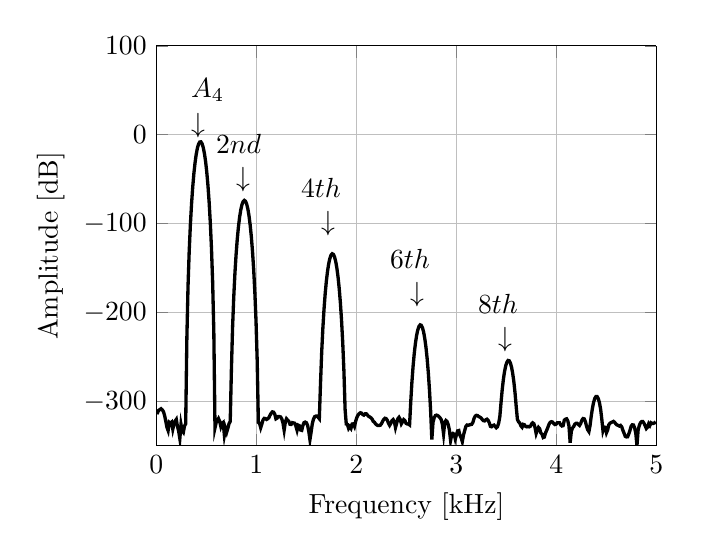
\begin{tikzpicture}

\begin{axis}[%
width=2.5in,
height=2in,
at={(2.6in,1.105in)},
scale only axis,
separate axis lines,
every outer x axis line/.append style={black},
every x tick label/.append style={font=\color{black}},
xmin=0,
xmax=5000,
xlabel={Frequency [kHz]},
ylabel={Amplitude [dB]},
xmajorgrids,
every outer y axis line/.append style={black},
every y tick label/.append style={font=\color{black}},
xticklabels={0, 1, 2, 3, 4, 5},
xtick={0, 1000, 2000, 3000, 4000, 5000},
ymin=-350,
ymax=100,
ymajorgrids,
axis background/.style={fill=white}
]
\addplot [color=black,solid,line width=1.2pt,forget plot]
  table[row sep=crcr]{%
0	-312.393016302885\\
11.7216117216117	-312.750583455041\\
23.4432234432234	-309.994565050399\\
35.1648351648352	-309.237655194648\\
46.8864468864469	-308.261829844295\\
58.6080586080586	-309.52985096643\\
70.3296703296703	-311.415193197503\\
82.0512820512821	-315.834122833724\\
93.7728937728938	-322.212259907834\\
105.494505494505	-329.219610996018\\
117.216117216117	-332.811470030214\\
128.937728937729	-323.616543339189\\
140.659340659341	-324.702381430647\\
152.380952380952	-323.426802414616\\
164.102564102564	-331.2775609663\\
175.824175824176	-325.282243066387\\
187.545787545788	-322.224246925756\\
199.267399267399	-320.28394289903\\
210.989010989011	-328.408983848227\\
222.710622710623	-333.38030904551\\
234.432234432234	-341.853998255673\\
246.153846153846	-325.99783354277\\
257.875457875458	-333.115601051128\\
269.59706959707	-334.821431460817\\
281.318681318681	-327.6792555811\\
293.040293040293	-325.121886852508\\
304.761904761905	-229.070012348246\\
316.483516483517	-170.096710589092\\
328.205128205128	-130.99278401216\\
339.92673992674	-101.341746863624\\
351.648351648352	-77.8235451673862\\
363.369963369963	-58.862347928062\\
375.091575091575	-43.5682874822595\\
386.813186813187	-31.3887524238473\\
398.534798534799	-21.9620577590889\\
410.25641025641	-15.0465146983279\\
421.978021978022	-10.4828441398642\\
433.699633699634	-8.17337826796222\\
445.421245421245	-8.07078476917002\\
457.142857142857	-10.1729924322429\\
468.864468864469	-14.5229748135592\\
480.586080586081	-21.2133368614159\\
492.307692307692	-30.3969107754678\\
504.029304029304	-42.3064425803193\\
515.750915750916	-57.2901203326941\\
527.472527472527	-75.8782177620287\\
539.194139194139	-98.9191674017364\\
550.915750915751	-127.898503780155\\
562.637362637363	-165.878917750715\\
574.358974358974	-221.916788901698\\
586.080586080586	-329.826183354317\\
597.802197802198	-323.957408086731\\
609.52380952381	-321.719169143043\\
621.245421245421	-319.387346172467\\
632.967032967033	-322.407352234819\\
644.688644688645	-328.340786180143\\
656.410256410256	-324.700658114868\\
668.131868131868	-323.652958513855\\
679.85347985348	-337.891948552159\\
691.575091575092	-330.563879545158\\
703.296703296703	-334.647907967722\\
715.018315018315	-330.243435426415\\
726.739926739927	-325.010800809723\\
738.461538461538	-322.630164365443\\
750.18315018315	-264.388115460561\\
761.904761904762	-216.861548669363\\
773.626373626374	-182.663005923388\\
785.347985347985	-156.058069003873\\
797.069597069597	-134.74759337614\\
808.791208791209	-117.534045803462\\
820.512820512821	-103.706686059208\\
832.234432234432	-92.8115678228919\\
843.956043956044	-84.5476310218852\\
855.677655677656	-78.7139565304939\\
867.399267399267	-75.1810917557384\\
879.120879120879	-73.8751634011121\\
890.842490842491	-74.7696796554579\\
902.564102564103	-77.8827399945924\\
914.285714285714	-83.2789330089498\\
926.007326007326	-91.0764084876735\\
937.728937728938	-101.461054440097\\
949.450549450549	-114.712187750017\\
961.172161172161	-131.249445314056\\
972.893772893773	-151.72367716364\\
984.615384615385	-177.212960721871\\
996.336996336996	-209.724472510411\\
1008.05860805861	-253.936832969581\\
1019.78021978022	-323.739860295081\\
1031.50183150183	-324.728356391827\\
1043.22344322344	-329.622873087564\\
1054.94505494505	-325.442839700976\\
1066.66666666667	-320.851423421034\\
1078.38827838828	-319.095167454806\\
1090.10989010989	-319.388202038003\\
1101.8315018315	-320.335400001491\\
1113.55311355311	-319.521645434165\\
1125.27472527473	-318.194154458228\\
1136.99633699634	-315.421056826497\\
1148.71794871795	-313.24132735901\\
1160.43956043956	-311.821173363448\\
1172.16117216117	-312.195261885358\\
1183.88278388278	-314.37106393182\\
1195.6043956044	-319.656073275685\\
1207.32600732601	-318.885123239098\\
1219.04761904762	-317.034702031628\\
1230.76923076923	-317.139262648469\\
1242.49084249084	-317.536379664312\\
1254.21245421245	-319.764487856463\\
1265.93406593407	-324.33031379908\\
1277.65567765568	-332.412228113015\\
1289.37728937729	-323.479036859072\\
1301.0989010989	-319.592283515592\\
1312.82051282051	-321.100243898777\\
1324.54212454212	-322.441923830058\\
1336.26373626374	-325.808880812572\\
1347.98534798535	-325.938535367664\\
1359.70695970696	-323.940132057621\\
1371.42857142857	-324.320400964702\\
1383.15018315018	-324.598076090416\\
1394.87179487179	-327.777917995524\\
1406.59340659341	-332.422193508061\\
1418.31501831502	-326.75910114996\\
1430.03663003663	-327.463166814816\\
1441.75824175824	-332.1760036073\\
1453.47985347985	-332.597051766038\\
1465.20146520147	-327.021190009344\\
1476.92307692308	-323.873715114686\\
1488.64468864469	-323.312817803593\\
1500.3663003663	-324.086052737173\\
1512.08791208791	-327.028287413878\\
1523.80952380952	-333.509402062438\\
1535.53113553114	-343.030672525587\\
1547.25274725275	-334.681968110489\\
1558.97435897436	-325.254973552374\\
1570.69597069597	-320.159599752367\\
1582.41758241758	-317.264743405266\\
1594.13919413919	-316.5792202439\\
1605.86080586081	-316.573930831755\\
1617.58241758242	-317.914574284885\\
1629.30402930403	-319.500065095323\\
1641.02564102564	-280.610249787516\\
1652.74725274725	-245.483360583091\\
1664.46886446886	-218.292805381144\\
1676.19047619048	-196.549370413148\\
1687.91208791209	-178.98874099033\\
1699.6336996337	-164.867514233589\\
1711.35531135531	-153.71332685409\\
1723.07692307692	-145.213596275151\\
1734.79853479853	-139.159530607706\\
1746.52014652015	-135.415827048023\\
1758.24175824176	-133.903867563543\\
1769.96336996337	-134.59293036285\\
1781.68498168498	-137.49694495119\\
1793.40659340659	-142.675950377823\\
1805.12820512821	-150.242629390836\\
1816.84981684982	-160.375686667279\\
1828.57142857143	-173.344170057312\\
1840.29304029304	-189.551718782595\\
1852.01465201465	-209.621694443407\\
1863.73626373626	-234.578600074395\\
1875.45787545788	-266.305264988195\\
1887.17948717949	-309.249327062903\\
1898.9010989011	-325.558223095414\\
1910.62271062271	-326.004351003493\\
1922.34432234432	-330.395826714921\\
1934.06593406593	-328.44405737144\\
1945.78754578755	-330.345117306161\\
1957.50915750916	-325.480504253811\\
1969.23076923077	-325.287403174369\\
1980.95238095238	-328.150580157216\\
1992.67399267399	-322.456738567737\\
2004.3956043956	-318.217478275396\\
2016.11721611722	-315.367737916279\\
2027.83882783883	-313.804255696911\\
2039.56043956044	-312.8147441227\\
2051.28205128205	-313.204628178701\\
2063.00366300366	-314.703298847107\\
2074.72527472527	-315.474850554067\\
2086.44688644689	-314.057043853359\\
2098.1684981685	-313.938880317369\\
2109.89010989011	-315.299910637299\\
2121.61172161172	-316.784223487067\\
2133.33333333333	-317.481630547156\\
2145.05494505495	-318.388724616478\\
2156.77655677656	-319.85238237128\\
2168.49816849817	-322.48172568237\\
2180.21978021978	-323.462546515932\\
2191.94139194139	-325.409767717203\\
2203.663003663	-326.46170134188\\
2215.38461538462	-327.169942681829\\
2227.10622710623	-327.083010867128\\
2238.82783882784	-326.8995865204\\
2250.54945054945	-325.165470176835\\
2262.27106227106	-322.421952191422\\
2273.99267399267	-320.226186541252\\
2285.71428571429	-319.005729391293\\
2297.4358974359	-319.389146742098\\
2309.15750915751	-321.288480518154\\
2320.87912087912	-324.530707139184\\
2332.60073260073	-326.983125357377\\
2344.32234432234	-324.74258802778\\
2356.04395604396	-321.628608895251\\
2367.76556776557	-320.469823554718\\
2379.48717948718	-322.6704629256\\
2391.20879120879	-329.475856435315\\
2402.9304029304	-324.684897604002\\
2414.65201465201	-319.527972398233\\
2426.37362637363	-317.904674190064\\
2438.09523809524	-320.216861797107\\
2449.81684981685	-325.195279249543\\
2461.53846153846	-322.998628293006\\
2473.26007326007	-320.520447619859\\
2484.98168498168	-321.594734078679\\
2496.7032967033	-324.756994024685\\
2508.42490842491	-325.379936582442\\
2520.14652014652	-325.480889650072\\
2531.86813186813	-326.475516932415\\
2543.58974358974	-300.686036785899\\
2555.31135531136	-278.387998730964\\
2567.03296703297	-260.472476777137\\
2578.75457875458	-246.053755385883\\
2590.47619047619	-234.638016832759\\
2602.1978021978	-225.900772321079\\
2613.91941391941	-219.625166077138\\
2625.64102564103	-215.669947679315\\
2637.36263736264	-213.951686667404\\
2649.08424908425	-214.435409233674\\
2660.80586080586	-217.130883202523\\
2672.52747252747	-222.093656054987\\
2684.24908424908	-229.431036012505\\
2695.9706959707	-239.314760733021\\
2707.69230769231	-252.004088642713\\
2719.41391941392	-267.886086954734\\
2731.13553113553	-287.537203332875\\
2742.85714285714	-311.579196554146\\
2754.57875457875	-342.959932666246\\
2766.30036630037	-323.525547867989\\
2778.02197802198	-318.543161971345\\
2789.74358974359	-315.988176026572\\
2801.4652014652	-315.479261367511\\
2813.18681318681	-315.970604823748\\
2824.90842490842	-317.029835075257\\
2836.63003663004	-318.536763586579\\
2848.35164835165	-320.531223560511\\
2860.07326007326	-325.972449274882\\
2871.79487179487	-336.559424910245\\
2883.51648351648	-323.828195443175\\
2895.2380952381	-321.540393396084\\
2906.95970695971	-322.734211172604\\
2918.68131868132	-326.26403753798\\
2930.40293040293	-332.367407292872\\
2942.12454212454	-343.96778698951\\
2953.84615384615	-337.354046681643\\
2965.56776556777	-336.062357088863\\
2977.28937728938	-336.808204934544\\
2989.01098901099	-342.349198570534\\
3000.7326007326	-337.734375571645\\
3012.45421245421	-333.192476881861\\
3024.17582417582	-332.825136408205\\
3035.89743589744	-338.338876753776\\
3047.61904761905	-340.962666815763\\
3059.34065934066	-345.241021227057\\
3071.06227106227	-337.88294939098\\
3082.78388278388	-333.058369599769\\
3094.50549450549	-328.266489588913\\
3106.22710622711	-326.605725678199\\
3117.94871794872	-326.826431953263\\
3129.67032967033	-326.642929146024\\
3141.39194139194	-325.932387676489\\
3153.11355311355	-325.853256740049\\
3164.83516483517	-323.778254780277\\
3176.55677655678	-319.212567754235\\
3188.27838827839	-316.566846265055\\
3200	-315.727465334911\\
3211.72161172161	-316.010123358911\\
3223.44322344322	-317.10915725921\\
3235.16483516484	-317.754707702736\\
3246.88644688645	-318.578095919227\\
3258.60805860806	-320.422428034343\\
3270.32967032967	-321.708120771122\\
3282.05128205128	-321.972667635789\\
3293.77289377289	-320.77798440487\\
3305.49450549451	-320.09766767378\\
3317.21611721612	-321.306852668847\\
3328.93772893773	-324.110594108306\\
3340.65934065934	-328.133484482567\\
3352.38095238095	-328.553648934747\\
3364.10256410256	-327.172507504316\\
3375.82417582418	-326.665332689459\\
3387.54578754579	-328.25478580404\\
3399.2673992674	-329.678220311715\\
3410.98901098901	-328.55219896569\\
3422.71062271062	-324.603624799471\\
3434.43223443223	-317.262873966919\\
3446.15384615385	-301.758742752465\\
3457.87545787546	-287.301890756105\\
3469.59706959707	-275.607497382808\\
3481.31868131868	-266.62013384802\\
3493.04029304029	-260.116093155687\\
3504.7619047619	-255.945755161113\\
3516.48351648352	-254.019544051965\\
3528.20512820513	-254.297918605493\\
3539.92673992674	-256.786044649775\\
3551.64835164835	-261.535813254344\\
3563.36996336996	-268.651699002498\\
3575.09157509158	-278.311244352527\\
3586.81318681319	-290.776036104204\\
3598.5347985348	-306.155270392879\\
3610.25641025641	-320.301940883581\\
3621.97802197802	-323.035463415248\\
3633.69963369963	-324.235039784383\\
3645.42124542125	-327.624064889382\\
3657.14285714286	-329.146739783512\\
3668.86446886447	-325.864360114328\\
3680.58608058608	-326.326988959226\\
3692.30769230769	-328.205997830588\\
3704.0293040293	-328.655251401501\\
3715.75091575092	-328.246075416461\\
3727.47252747253	-328.691853079297\\
3739.19413919414	-328.081942089057\\
3750.91575091575	-325.533495689787\\
3762.63736263736	-324.160918296521\\
3774.35897435897	-325.114512644882\\
3786.08058608059	-329.12211821853\\
3797.8021978022	-336.125058050113\\
3809.52380952381	-332.390474443368\\
3821.24542124542	-329.341710183504\\
3832.96703296703	-330.837624593429\\
3844.68864468864	-335.581660581079\\
3856.41025641026	-336.911079902605\\
3868.13186813187	-340.724569734202\\
3879.85347985348	-340.145607031333\\
3891.57509157509	-335.423482161887\\
3903.2967032967	-332.524527308962\\
3915.01831501832	-329.187184962008\\
3926.73992673993	-325.682433365116\\
3938.46153846154	-323.514976782424\\
3950.18315018315	-322.885830561374\\
3961.90476190476	-323.26540084032\\
3973.62637362637	-324.984003264706\\
3985.34798534799	-326.0334837034\\
3997.0695970696	-325.669185014251\\
4008.79120879121	-324.04974357776\\
4020.51282051282	-324.010732189018\\
4032.23443223443	-324.052690431885\\
4043.95604395604	-326.620685593304\\
4055.67765567766	-327.719530739473\\
4067.39926739927	-327.318438214878\\
4079.12087912088	-321.259009420026\\
4090.84249084249	-320.015608078248\\
4102.5641025641	-319.671924746435\\
4114.28571428571	-321.901816290655\\
4126.00732600733	-327.706822246467\\
4137.72893772894	-346.483652647309\\
4149.45054945055	-333.742766718489\\
4161.17216117216	-329.902456613246\\
4172.89377289377	-328.316832562793\\
4184.61538461538	-325.652221398136\\
4196.336996337	-324.726280148115\\
4208.05860805861	-324.679136734137\\
4219.78021978022	-325.9155653929\\
4231.50183150183	-327.075878344186\\
4243.22344322344	-324.91190494745\\
4254.94505494505	-321.201646174634\\
4266.66666666667	-319.366066524567\\
4278.38827838828	-319.671867628567\\
4290.10989010989	-322.734728364904\\
4301.8315018315	-328.213655500157\\
4313.55311355311	-332.009646381184\\
4325.27472527472	-333.961355348029\\
4336.99633699634	-326.937841902107\\
4348.71794871795	-316.541372081428\\
4360.43956043956	-307.803456495246\\
4372.16117216117	-301.162205095561\\
4383.88278388278	-296.703255203503\\
4395.6043956044	-294.517214792388\\
4407.32600732601	-294.582602759188\\
4419.04761904762	-296.90198036475\\
4430.76923076923	-301.578528302874\\
4442.49084249084	-308.880098512925\\
4454.21245421245	-320.100048587643\\
4465.93406593407	-333.001241402038\\
4477.65567765568	-328.947501712991\\
4489.37728937729	-329.182296221414\\
4501.0989010989	-335.244547541631\\
4512.82051282051	-332.099288936681\\
4524.54212454212	-326.308418440831\\
4536.26373626374	-324.567953401431\\
4547.98534798535	-323.777417140646\\
4559.70695970696	-323.175338947132\\
4571.42857142857	-322.532457241576\\
4583.15018315018	-323.6689025953\\
4594.87179487179	-325.342244976187\\
4606.59340659341	-326.574026559655\\
4618.31501831502	-327.0050454052\\
4630.03663003663	-327.790390538844\\
4641.75824175824	-327.071561360584\\
4653.47985347985	-328.694100975977\\
4665.20146520147	-332.544654794148\\
4676.92307692308	-335.872406290806\\
4688.64468864469	-339.314007124611\\
4700.3663003663	-339.952049349337\\
4712.08791208791	-339.874065788702\\
4723.80952380952	-336.656904180176\\
4735.53113553114	-332.764298655737\\
4747.25274725275	-328.081673635743\\
4758.97435897436	-326.34367685237\\
4770.69597069597	-326.558648261231\\
4782.41758241758	-329.789430379892\\
4794.13919413919	-335.907293785548\\
4805.86080586081	-349.690610325123\\
4817.58241758242	-332.066074729122\\
4829.30402930403	-327.149466119118\\
4841.02564102564	-323.964163519787\\
4852.74725274725	-322.792804289577\\
4864.46886446886	-322.694630410178\\
4876.19047619048	-324.599972298664\\
4887.91208791209	-327.442433419968\\
4899.6336996337	-330.547218380715\\
4911.35531135531	-329.120005198479\\
4923.07692307692	-325.172127931692\\
4934.79853479854	-327.136886355979\\
4946.52014652015	-324.078291396898\\
4958.24175824176	-324.791895728033\\
4969.96336996337	-324.776197468661\\
4981.68498168498	-324.203323930703\\
4993.40659340659	-322.990827703511\\
};
\node[right, align=left, text=black] at (axis cs:250,10) {$\downarrow$};
\node[right, align=left, text=black] at (axis cs:250,50) {\text{$A_4$}};

\node[right, align=left, text=black] at (axis cs:700,-50) {$\downarrow$};
\node[right, align=left, text=black] at (axis cs:500,-10) {$\text{2nd}$};

\node[right, align=left, text=black] at (axis cs:1550,-100) {$\downarrow$};
\node[right, align=left, text=black] at (axis cs:1350,-60) {$\text{4th}$};

\node[right, align=left, text=black] at (axis cs:2440,-180) {$\downarrow$};
\node[right, align=left, text=black] at (axis cs:2240,-140) {$\text{6th}$};

\node[right, align=left, text=black] at (axis cs:3320,-230) {$\downarrow$};
\node[right, align=left, text=black] at (axis cs:3120,-190) {$\text{8th}$};

\end{axis}
\end{tikzpicture}%
	\caption{A signal consisting of multiple even harmonics}
	\label{fig:EvenTHD}
\end{subfigure}
\hspace{6mm} 
\begin{subfigure}[t]{0.47\textwidth}
	\tikzsetnextfilename{OddTHD}
	% This file was created by matlab2tikz.
%
%The latest updates can be retrieved from
%  http://www.mathworks.com/matlabcentral/fileexchange/22022-matlab2tikz-matlab2tikz
%where you can also make suggestions and rate matlab2tikz.
%
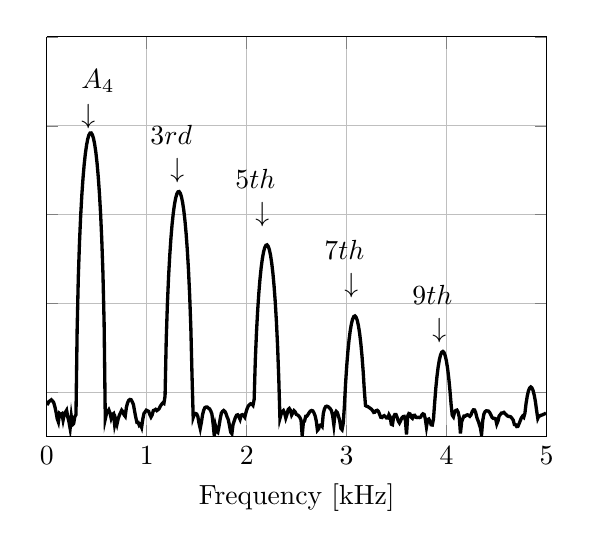
\begin{tikzpicture}

\begin{axis}[%
width=2.5in,
height=2in,
at={(2.6in,1.105in)},
scale only axis,
separate axis lines,
every outer x axis line/.append style={black},
every x tick label/.append style={font=\color{black}},
xmin=0,
xmax=5000,
xlabel={Frequency [kHz]},
xticklabels={0, 1, 2, 3, 4, 5},
xtick={0, 1000, 2000, 3000, 4000, 5000},
xmajorgrids,
every outer y axis line/.append style={black},
every y tick label/.append style={font=\color{black}},
ymin=-350,
ymax=100,
ymajorgrids,
yticklabels={\empty},
axis background/.style={fill=white}
]
\addplot [color=black,solid,line width=1.2pt,forget plot]
  table[row sep=crcr]{%
0	-312.476774360719\\
11.7216117216117	-312.76063985607\\
23.4432234432234	-310.046834057316\\
35.1648351648352	-309.409238406673\\
46.8864468864469	-308.213692663403\\
58.6080586080586	-309.551022302417\\
70.3296703296703	-311.368850463978\\
82.0512820512821	-316.013736294795\\
93.7728937728938	-322.066424944641\\
105.494505494505	-329.587315271092\\
117.216117216117	-333.301375126281\\
128.937728937729	-323.704515145192\\
140.659340659341	-324.870526088801\\
152.380952380952	-323.947138226521\\
164.102564102564	-331.184758306792\\
175.824175824176	-324.915285525654\\
187.545787545788	-322.196194096509\\
199.267399267399	-320.015150056997\\
210.989010989011	-327.676348231159\\
222.710622710623	-333.12661516104\\
234.432234432234	-340.484086317907\\
246.153846153846	-326.933152445235\\
257.875457875458	-336.30263836172\\
269.59706959707	-335.033227686605\\
281.318681318681	-327.244352888687\\
293.040293040293	-325.02108577898\\
304.761904761905	-229.070024421709\\
316.483516483517	-170.096710568549\\
328.205128205128	-130.992784012266\\
339.92673992674	-101.341746863623\\
351.648351648352	-77.8235451673866\\
363.369963369963	-58.862347928062\\
375.091575091575	-43.5682874822595\\
386.813186813187	-31.3887524238473\\
398.534798534799	-21.9620577590889\\
410.25641025641	-15.0465146983279\\
421.978021978022	-10.4828441398642\\
433.699633699634	-8.17337826796222\\
445.421245421245	-8.07078476917002\\
457.142857142857	-10.1729924322429\\
468.864468864469	-14.5229748135592\\
480.586080586081	-21.2133368614159\\
492.307692307692	-30.3969107754678\\
504.029304029304	-42.3064425803193\\
515.750915750916	-57.2901203326941\\
527.472527472527	-75.8782177620287\\
539.194139194139	-98.9191674017364\\
550.915750915751	-127.898503780138\\
562.637362637363	-165.878917748157\\
574.358974358974	-221.916787431611\\
586.080586080586	-329.860262269524\\
597.802197802198	-323.920056274176\\
609.52380952381	-321.777760271602\\
621.245421245421	-319.56378804444\\
632.967032967033	-322.955130594619\\
644.688644688645	-328.902783824495\\
656.410256410256	-324.81324369016\\
668.131868131868	-323.824579696544\\
679.85347985348	-336.443363291767\\
691.575091575092	-330.958189746236\\
703.296703296703	-335.635303825514\\
715.018315018315	-329.687484999979\\
726.739926739927	-325.608033556523\\
738.461538461538	-322.882069629021\\
750.18315018315	-319.966421030175\\
761.904761904762	-321.652510574295\\
773.626373626374	-325.143097235804\\
785.347985347985	-326.879168570855\\
797.069597069597	-316.896335178847\\
808.791208791209	-311.74488212211\\
820.512820512821	-308.878013137209\\
832.234432234432	-307.917832678248\\
843.956043956044	-308.142177517833\\
855.677655677656	-310.48290310127\\
867.399267399267	-313.566789813448\\
879.120879120879	-320.954843742391\\
890.842490842491	-327.965127694527\\
902.564102564103	-333.697564101067\\
914.285714285714	-333.641015172163\\
926.007326007326	-336.986224889743\\
937.728937728938	-335.689770286189\\
949.450549450549	-339.096181030464\\
961.172161172161	-330.073394693885\\
972.893772893773	-323.635297508999\\
984.615384615385	-321.849732327126\\
996.336996336996	-319.966414107395\\
1008.05860805861	-320.709857474733\\
1019.78021978022	-321.300669127717\\
1031.50183150183	-324.82957280474\\
1043.22344322344	-327.621154108766\\
1054.94505494505	-325.268479455014\\
1066.66666666667	-320.350341747414\\
1078.38827838828	-319.876449266419\\
1090.10989010989	-319.014194670653\\
1101.8315018315	-320.392503492053\\
1113.55311355311	-319.366162724767\\
1125.27472527473	-318.161837020659\\
1136.99633699634	-315.400404949723\\
1148.71794871795	-313.356081371107\\
1160.43956043956	-311.884613942132\\
1172.16117216117	-312.499118660274\\
1183.88278388278	-303.906248686671\\
1195.6043956044	-240.487683459538\\
1207.32600732601	-200.186666481123\\
1219.04761904762	-169.837303457185\\
1230.76923076923	-145.828724060088\\
1242.49084249084	-126.48689333498\\
1254.21245421245	-110.877732145859\\
1265.93406593407	-98.425090812862\\
1277.65567765568	-88.7531956748779\\
1289.37728937729	-81.6110984418175\\
1301.0989010989	-76.8328967329348\\
1312.82051282051	-74.3157638673602\\
1324.54212454212	-74.0079654791933\\
1336.26373626374	-75.9032860875509\\
1347.98534798535	-80.0403796303048\\
1359.70695970696	-86.5068784217325\\
1371.42857142857	-95.4493347836206\\
1383.15018315018	-107.091851581825\\
1394.87179487179	-121.76967655037\\
1406.59340659341	-139.99186438544\\
1418.31501831502	-162.567961382642\\
1430.03663003663	-190.900287110181\\
1441.75824175824	-227.822096243241\\
1453.47985347985	-281.270740748748\\
1465.20146520147	-328.097999339852\\
1476.92307692308	-324.316162999833\\
1488.64468864469	-323.683212362215\\
1500.3663003663	-324.298281103684\\
1512.08791208791	-327.288612001059\\
1523.80952380952	-334.933889260514\\
1535.53113553114	-340.568470088625\\
1547.25274725275	-333.558297453405\\
1558.97435897436	-325.09610629774\\
1570.69597069597	-319.846400442748\\
1582.41758241758	-317.010589907898\\
1594.13919413919	-316.348060250503\\
1605.86080586081	-316.450564453629\\
1617.58241758242	-317.652002975581\\
1629.30402930403	-318.472767093789\\
1641.02564102564	-320.861617465552\\
1652.74725274725	-324.447114626559\\
1664.46886446886	-335.439977747053\\
1676.19047619048	-348.924463490367\\
1687.91208791209	-337.82752617514\\
1699.6336996337	-343.579887627296\\
1711.35531135531	-344.819403421232\\
1723.07692307692	-338.323072830193\\
1734.79853479853	-330.036092150647\\
1746.52014652015	-323.354919028514\\
1758.24175824176	-321.282712178017\\
1769.96336996337	-320.264687118138\\
1781.68498168498	-321.322836018848\\
1793.40659340659	-323.763863752341\\
1805.12820512821	-327.714829983451\\
1816.84981684982	-330.818868464947\\
1828.57142857143	-337.547955969765\\
1840.29304029304	-344.800859253392\\
1852.01465201465	-346.446727708821\\
1863.73626373626	-335.961437480006\\
1875.45787545788	-332.024277725398\\
1887.17948717949	-328.257649771995\\
1898.9010989011	-325.582749555652\\
1910.62271062271	-325.180917678106\\
1922.34432234432	-327.289009152216\\
1934.06593406593	-330.278330929783\\
1945.78754578755	-325.493273209383\\
1957.50915750916	-324.984636918903\\
1969.23076923077	-325.705126654008\\
1980.95238095238	-327.681066815279\\
1992.67399267399	-322.562337255015\\
2004.3956043956	-318.223664116799\\
2016.11721611722	-315.324356143881\\
2027.83882783883	-313.742654653434\\
2039.56043956044	-312.727704717282\\
2051.28205128205	-313.141092601404\\
2063.00366300366	-314.528443301922\\
2074.72527472527	-307.911732425111\\
2086.44688644689	-263.468672573293\\
2098.1684981685	-232.367038324986\\
2109.89010989011	-207.853514575446\\
2121.61172161172	-188.123117404742\\
2133.33333333333	-172.193936717314\\
2145.05494505495	-159.464966014383\\
2156.77655677656	-149.545711420736\\
2168.49816849817	-142.175629941949\\
2180.21978021978	-137.182009653397\\
2191.94139194139	-134.456763008031\\
2203.663003663	-133.943706039296\\
2215.38461538462	-135.63247345012\\
2227.10622710623	-139.557434626185\\
2238.82783882784	-145.801333928684\\
2250.54945054945	-154.50460192328\\
2262.27106227106	-165.8829817437\\
2273.99267399267	-180.259304251735\\
2285.71428571429	-198.122444416711\\
2297.4358974359	-220.245355231257\\
2309.15750915751	-247.952569423375\\
2320.87912087912	-283.84707169342\\
2332.60073260073	-329.220953136781\\
2344.32234432234	-324.410043915768\\
2356.04395604396	-321.59146892775\\
2367.76556776557	-320.35614411151\\
2379.48717948718	-323.270729744722\\
2391.20879120879	-328.745422163443\\
2402.9304029304	-324.890399353977\\
2414.65201465201	-319.245398021764\\
2426.37362637363	-318.029931553817\\
2438.09523809524	-320.094691431967\\
2449.81684981685	-325.440299359182\\
2461.53846153846	-323.094219605479\\
2473.26007326007	-320.600604413651\\
2484.98168498168	-321.858484668915\\
2496.7032967033	-324.746680244289\\
2508.42490842491	-325.324298319437\\
2520.14652014652	-326.434251142161\\
2531.86813186813	-328.093941575175\\
2543.58974358974	-331.181578566255\\
2555.31135531136	-348.648017613807\\
2567.03296703297	-333.351605972041\\
2578.75457875458	-332.276114687494\\
2590.47619047619	-326.815503070475\\
2602.1978021978	-326.66606253933\\
2613.91941391941	-324.852134638865\\
2625.64102564103	-322.568385395915\\
2637.36263736264	-320.909516305782\\
2649.08424908425	-320.294198082906\\
2660.80586080586	-320.7370860187\\
2672.52747252747	-322.890274439618\\
2684.24908424908	-326.233425462405\\
2695.9706959707	-332.0108040271\\
2707.69230769231	-342.589148702971\\
2719.41391941392	-341.063298400802\\
2731.13553113553	-336.951008034904\\
2742.85714285714	-336.521772442751\\
2754.57875457875	-338.141378834923\\
2766.30036630037	-323.672731783199\\
2778.02197802198	-318.506069316446\\
2789.74358974359	-315.950843004944\\
2801.4652014652	-315.458996443669\\
2813.18681318681	-315.91747965454\\
2824.90842490842	-317.082960686894\\
2836.63003663004	-318.437130343247\\
2848.35164835165	-320.609923195954\\
2860.07326007326	-326.373271932224\\
2871.79487179487	-336.548979902884\\
2883.51648351648	-324.182122753493\\
2895.2380952381	-321.369650398793\\
2906.95970695971	-322.616452248608\\
2918.68131868132	-326.88841632779\\
2930.40293040293	-331.747417435161\\
2942.12454212454	-340.465344649171\\
2953.84615384615	-341.929658858457\\
2965.56776556777	-334.714944917966\\
2977.28937728938	-315.305710631703\\
2989.01098901099	-289.948132227998\\
3000.7326007326	-269.794345810704\\
3012.45421245421	-253.538058562358\\
3024.17582417582	-240.529242846707\\
3035.89743589744	-230.3603737732\\
3047.61904761905	-222.760813871235\\
3059.34065934066	-217.550845904535\\
3071.06227106227	-214.616997436478\\
3082.78388278388	-213.898587590974\\
3094.50549450549	-215.381091252002\\
3106.22710622711	-219.094618891038\\
3117.94871794872	-225.117088010747\\
3129.67032967033	-233.582932890879\\
3141.39194139194	-244.699539271444\\
3153.11355311355	-258.775678613699\\
3164.83516483517	-276.254814234603\\
3176.55677655678	-297.440570072309\\
3188.27838827839	-314.806326093219\\
3200	-315.556709803705\\
3211.72161172161	-315.925716382722\\
3223.44322344322	-316.941299690089\\
3235.16483516484	-317.811985388593\\
3246.88644688645	-318.757124994702\\
3258.60805860806	-320.298744036523\\
3270.32967032967	-322.478725700834\\
3282.05128205128	-322.20165869146\\
3293.77289377289	-320.503182232187\\
3305.49450549451	-320.06732847349\\
3317.21611721612	-321.23227949997\\
3328.93772893773	-324.463473006262\\
3340.65934065934	-327.912645445808\\
3352.38095238095	-328.201158145493\\
3364.10256410256	-326.843951092668\\
3375.82417582418	-326.127439838193\\
3387.54578754579	-327.376937115064\\
3399.2673992674	-328.796189959288\\
3410.98901098901	-328.828502947131\\
3422.71062271062	-325.034964266974\\
3434.43223443223	-327.456722230403\\
3446.15384615385	-335.718110030268\\
3457.87545787546	-336.318635966039\\
3469.59706959707	-327.296557357219\\
3481.31868131868	-324.763344589083\\
3493.04029304029	-324.76211602158\\
3504.7619047619	-328.077405552291\\
3516.48351648352	-332.291951156579\\
3528.20512820513	-334.40610252494\\
3539.92673992674	-331.803308083215\\
3551.64835164835	-328.537344340231\\
3563.36996336996	-327.188172465112\\
3575.09157509158	-326.922146012165\\
3586.81318681319	-331.121447859404\\
3598.5347985348	-347.184604321136\\
3610.25641025641	-326.626029520201\\
3621.97802197802	-323.706851177176\\
3633.69963369963	-324.140738344225\\
3645.42124542125	-327.910051158916\\
3657.14285714286	-329.122613649713\\
3668.86446886447	-325.838512480764\\
3680.58608058608	-325.679715106915\\
3692.30769230769	-327.974623481713\\
3704.0293040293	-328.265649526291\\
3715.75091575092	-327.919763605474\\
3727.47252747253	-328.290278843386\\
3739.19413919414	-327.787819956943\\
3750.91575091575	-325.446980413527\\
3762.63736263736	-324.068479837798\\
3774.35897435897	-324.664965607256\\
3786.08058608059	-329.406710421099\\
3797.8021978022	-338.713999427433\\
3809.52380952381	-330.481253817979\\
3821.24542124542	-329.852569727394\\
3832.96703296703	-332.685279710581\\
3844.68864468864	-336.404418876203\\
3856.41025641026	-336.640021637934\\
3868.13186813187	-329.704756216772\\
3879.85347985348	-311.803454287358\\
3891.57509157509	-295.00298948847\\
3903.2967032967	-281.642577234596\\
3915.01831501832	-271.204146173316\\
3926.73992673993	-263.369450911924\\
3938.46153846154	-257.941053158538\\
3950.18315018315	-254.797639320443\\
3961.90476190476	-253.873543755289\\
3973.62637362637	-255.149868408062\\
3985.34798534799	-258.651913760564\\
3997.0695970696	-264.451021516027\\
4008.79120879121	-272.672617200823\\
4020.51282051282	-283.491449439096\\
4032.23443223443	-297.053176629451\\
4043.95604395604	-313.097937695934\\
4055.67765567766	-325.580254986861\\
4067.39926739927	-327.434063099967\\
4079.12087912088	-322.215885644693\\
4090.84249084249	-320.246715731047\\
4102.5641025641	-319.831622724413\\
4114.28571428571	-322.057310550306\\
4126.00732600733	-327.934915811868\\
4137.72893772894	-346.158495614059\\
4149.45054945055	-333.313024604962\\
4161.17216117216	-329.486695106301\\
4172.89377289377	-326.52826484316\\
4184.61538461538	-326.654167659735\\
4196.336996337	-325.652683364245\\
4208.05860805861	-325.140453942067\\
4219.78021978022	-325.855081508886\\
4231.50183150183	-326.840172418474\\
4243.22344322344	-325.31320098108\\
4254.94505494505	-321.517261523122\\
4266.66666666667	-319.610279650183\\
4278.38827838828	-319.644539016795\\
4290.10989010989	-322.626217987192\\
4301.8315018315	-328.196237912869\\
4313.55311355311	-331.651145602864\\
4325.27472527472	-335.592058030827\\
4336.99633699634	-339.824216887629\\
4348.71794871795	-347.643174643096\\
4360.43956043956	-331.808622008623\\
4372.16117216117	-324.427001066957\\
4383.88278388278	-321.658677234437\\
4395.6043956044	-320.6640761508\\
4407.32600732601	-320.7659539727\\
4419.04761904762	-321.024341362508\\
4430.76923076923	-322.732651704794\\
4442.49084249084	-325.271581260597\\
4454.21245421245	-328.145282842489\\
4465.93406593407	-329.162026470824\\
4477.65567765568	-329.029124152688\\
4489.37728937729	-329.597183950017\\
4501.0989010989	-335.544802841813\\
4512.82051282051	-332.303891980705\\
4524.54212454212	-326.449850536787\\
4536.26373626374	-324.861552870403\\
4547.98534798535	-323.192784263351\\
4559.70695970696	-323.134882937047\\
4571.42857142857	-322.406994627788\\
4583.15018315018	-323.800809009745\\
4594.87179487179	-325.002287074804\\
4606.59340659341	-326.382632574176\\
4618.31501831502	-326.903686099408\\
4630.03663003663	-326.988865378937\\
4641.75824175824	-327.513134647041\\
4653.47985347985	-329.210369891362\\
4665.20146520147	-331.041516838604\\
4676.92307692308	-336.077200361121\\
4688.64468864469	-336.309065384227\\
4700.3663003663	-338.380657364757\\
4712.08791208791	-338.213633526287\\
4723.80952380952	-335.22398424552\\
4735.53113553114	-331.84909451913\\
4747.25274725275	-328.558484550391\\
4758.97435897436	-326.701649358589\\
4770.69597069597	-327.933249232296\\
4782.41758241758	-323.375710430514\\
4794.13919413919	-312.136823094276\\
4805.86080586081	-304.074795991442\\
4817.58241758242	-298.366282200733\\
4829.30402930403	-295.006431173174\\
4841.02564102564	-293.821913521472\\
4852.74725274725	-294.827530636422\\
4864.46886446886	-297.956204949545\\
4876.19047619048	-303.248744344501\\
4887.91208791209	-310.70739122936\\
4899.6336996337	-320.529953490212\\
4911.35531135531	-329.208039103346\\
4923.07692307692	-326.386496128955\\
4934.79853479854	-326.377861872946\\
4946.52014652015	-325.504414222792\\
4958.24175824176	-325.258658121801\\
4969.96336996337	-324.49947853918\\
4981.68498168498	-323.964753373818\\
4993.40659340659	-323.116477825657\\
};
\node[right, align=left, text=black] at (axis cs:250,10) {$\downarrow$};
\node[right, align=left, text=black] at (axis cs:250,50) {\text{$A_4$}};

\node[right, align=left, text=black] at (axis cs:1140,-50) {$\downarrow$};
\node[right, align=left, text=black] at (axis cs:940,-10) {$\text{3rd}$};

\node[right, align=left, text=black] at (axis cs:1990,-100) {$\downarrow$};
\node[right, align=left, text=black] at (axis cs:1790,-60) {$\text{5th}$};

\node[right, align=left, text=black] at (axis cs:2880,-180) {$\downarrow$};
\node[right, align=left, text=black] at (axis cs:2680,-140) {$\text{7th}$};

\node[right, align=left, text=black] at (axis cs:3760,-230) {$\downarrow$};
\node[right, align=left, text=black] at (axis cs:3560,-190) {$\text{9th}$};
\end{axis}
\end{tikzpicture}%
	\caption{A signal consisting of multiple odd harmonics}
	\label{fig:OddTHD}
\end{subfigure}
\caption{A Spectrum}
\end{figure}


\begin{table}[H]
\centering
\ra{1.3}
\begin{tabular}{S[table-format=1]ccccccc} \toprule
    {Harmonic} & {$A_2$} & {$A_3$} & {$A_4$} & {$A_5$} & {$A_6$} & {$A_7$} & {$A_8$} \\ \midrule 
    $F_o$  & 110  & 220  & \textcolor{red}{440}   & \textcolor{red}{880}  & \textcolor{red}{1760}  & \textcolor{red}{3520}   & 7040   \\ \bottomrule
    2      & 220  & 440  & \textcolor{red}{880}   & 1760 & 3520   & 7040   & 14080  \\ 
    3      & 330  & 660  & 1320  & 2640 & 5280   & 10560  & 21120  \\
    4      & 440  & 880  & \textcolor{red}{1760}  & 3520 & 7040   & 14080  & 28160  \\ 
    5      & 550  & 1100 & 2200  & 4400 & 8800   & 17600  & 35200  \\ \midrule
    6      & 660  & 1320 & 2640  & 5280 & 10560  & 21120  & 42240  \\
    7      & 770  & 1540 & 3080  & 6160 & 12320  & 24640  & 49280  \\
    8      & 880  & 1760 & \textcolor{red}{3520}  & 7040 & 14080  & 28160  & 56320  \\ 
    9      & 990  & 1980 & 3960  & 7920 & 15840  & 31680  & 63360  \\ \bottomrule
\end{tabular}
\caption{Table of A-note, $F_o$ , harmonics in accordance with their fundamental tone frequency. Every unit is in [Hz].\citep{sou:NoteA}}
\end{table}


